\documentclass[a4paper,twoside]{article}
\usepackage{blindtext}  
\usepackage{geometry}

% Chinese support
\usepackage[UTF8, scheme = plain]{ctex}

% Page margin layout
\geometry{left=2.3cm,right=2cm,top=2.5cm,bottom=2.0cm}


\usepackage{listings}
\usepackage{xcolor}
\usepackage{geometry}
\usepackage{amsmath}
\usepackage{float}
\usepackage{hyperref}

\usepackage{graphics}
\usepackage{graphicx}
\usepackage{epsfig}
\usepackage{float}
\usepackage{wrapfig}

\usepackage{algorithm}
\usepackage[noend]{algpseudocode}

\usepackage{booktabs}
\usepackage{threeparttable}
\usepackage{longtable}
\usepackage{listings}
\usepackage{tikz}
\usepackage{multicol}

\usepackage{caption}
\usepackage{subcaption}

% cite package, to clean up citations in the main text. Do not remove.
\usepackage{cite}

\usepackage{color,xcolor}

%% The amssymb package provides various useful mathematical symbols
\usepackage{amssymb}
%% The amsthm package provides extended theorem environments
\usepackage{amsthm}
\usepackage{amsfonts}
\usepackage{enumerate}
\usepackage{enumitem}
\usepackage{listings}

\usepackage{textcomp}

\usepackage{indentfirst}
\setlength{\parindent}{2em} % Make two letter space in the first paragraph
\usepackage{setspace}
\linespread{1.5} % Line spacing setting
\usepackage{siunitx}
\setlength{\parskip}{0.5em} % Paragraph spacing setting

% \usepackage[contents =22920202204622, scale = 10, color = black, angle = 50, opacity = .10]{background}

\renewcommand{\figurename}{图}
\renewcommand{\lstlistingname}{代码} 
\renewcommand{\tablename}{表格}
\renewcommand{\contentsname}{目录}
\floatname{algorithm}{算法}

\graphicspath{ {images/} }

%%%%%%%%%%%%%
\newcommand{\StudentNumber}{22920202204622}  % Fill your student number here
\newcommand{\StudentName}{熊恪峥}  % Replace your name here
\newcommand{\PaperTitle}{实验(四)}  % Change your paper title here
\newcommand{\PaperType}{计算机网络} % Replace the type of your report here
\newcommand{\Date}{2022年11月26日}
\newcommand{\College}{信息学院}
\newcommand{\CourseName}{计算机网络}
%%%%%%%%%%%%%

%% Page header and footer setting
\usepackage{fancyhdr}
\usepackage{lastpage}
\pagestyle{fancy}
\fancyhf{}
% This requires the document to be twoside
\fancyhead[LO]{\texttt{\StudentName }}
\fancyhead[LE]{\texttt{\StudentNumber}}
\fancyhead[C]{\texttt{\PaperTitle }}
\fancyhead[R]{\texttt{第{\thepage}页,共\pageref*{LastPage}页}}


\title{\PaperTitle}
\author{\StudentName}
\date{\Date}

\lstset{
	basicstyle          =   \sffamily,          % 基本代码风格
	keywordstyle        =   \bfseries,          % 关键字风格
	commentstyle        =   \rmfamily\itshape,  % 注释的风格,斜体
	stringstyle         =   \ttfamily,  % 字符串风格
	flexiblecolumns,                % 别问为什么,加上这个
	numbers             =   left,   % 行号的位置在左边
	showspaces          =   false,  % 是否显示空格,显示了有点乱,所以不现实了
	numberstyle         =   \zihao{-5}\ttfamily,    % 行号的样式,小五号,tt等宽字体
	showstringspaces    =   false,
	captionpos          =   t,      % 这段代码的名字所呈现的位置,t指的是top上面
	frame               =   lrtb,   % 显示边框
}

\lstdefinestyle{PythonStyle}{
	language        =   Python, % 语言选Python
	basicstyle      =   \zihao{-5}\ttfamily,
	numberstyle     =   \zihao{-5}\ttfamily,
	keywordstyle    =   \color{blue},
	keywordstyle    =   [2] \color{teal},
	stringstyle     =   \color{magenta},
	commentstyle    =   \color{red}\ttfamily,
	breaklines      =   true,   % 自动换行,建议不要写太长的行
	columns         =   fixed,  % 如果不加这一句,字间距就不固定,很丑,必须加
	basewidth       =   0.5em,
}

\definecolor{keycolor}{RGB}{172, 42, 42}
\definecolor{mbleu}{RGB}{64,96,127}
\definecolor{vimvert}{RGB}{46, 139, 87}

\lstdefinestyle{MakefileBaseStyle}{
basicstyle=\ttfamily\scriptsize\color{black!90},%
stringstyle=\itshape\color{magenta},%
showstringspaces=false,%
keywordstyle=\bfseries\color{keycolor},%
commentstyle=\color{blue}\slshape,%
framexleftmargin=1mm,%
backgroundcolor=\color{black!2},%
}

\lstdefinestyle{MakefileStyle}{
	otherkeywords={.SUFFIXES},
	morekeywords={SUFFIX, CPP_,},
	moredelim=[is][\color{mbleu}]{/*}{*/},
	style=MakefileBaseStyle,%
	morecomment=[l][commentstyle]{\#},%
	emphstyle={\color{vimvert}},%
	moredelim=[s][\color{vimvert}]{\$(}{)}%
}

\lstdefinestyle{CppStyle}{
	language        =   c++,
	basicstyle      =   \zihao{-5}\ttfamily,
	numberstyle     =   \zihao{-5}\ttfamily,
	keywordstyle    =   \color{blue},
	keywordstyle    =   [2] \color{teal},
	stringstyle     =   \color{magenta},
	commentstyle    =   \color{red}\ttfamily,
	breaklines      =   true,   % 自动换行,建议不要写太长的行
	columns         =   fixed,  % 如果不加这一句,字间距就不固定,很丑,必须加
	basewidth       =   0.5em,
}

\algnewcommand\algorithmicinput{\textbf{Input:}}
\algnewcommand\algorithmicoutput{\textbf{Output:}}
\algnewcommand\Input{\item[\algorithmicinput]}%
\algnewcommand\Output{\item[\algorithmicoutput]}%

\usetikzlibrary{positioning, shapes.geometric}

% 流程图定义基本形状
\tikzstyle{startstop} = [rectangle, rounded corners, minimum width = 2cm, minimum height=1cm,text centered, draw = black]
\tikzstyle{io} = [trapezium, trapezium left angle=70, trapezium right angle=110, minimum width=2cm, minimum height=1cm, text centered, draw=black]
\tikzstyle{process} = [rectangle, minimum width=3cm, minimum height=1cm, text centered, draw=black]
\tikzstyle{decision} = [diamond, aspect = 3, text centered, draw=black]
% 箭头形式
\tikzstyle{arrow} = [->,>=stealth]

\newtheorem{assumption}{Assumption}[section]

\begin{document}
	
%%%%%%%%%%%%%%%%%%%%%%%%%%%%%%%%%%%%%%%%%%%%
\makeatletter % change default title style
\renewcommand*\maketitle{%
	\begin{center} 
		\bfseries  % title 
		{\LARGE \@title \par}  % LARGE typesetting
		\vskip 1em  %  margin 1em
		{\global\let\author\@empty}  % no author information
		{\global\let\date\@empty}  % no date
		\thispagestyle{empty}   %  empty page style
	\end{center}%
	\setcounter{footnote}{0}%
}
\makeatother
%%%%%%%%%%%%%%%%%%%%%%%%%%%%%%%%%%%%%%%%%%%%
	
	
\thispagestyle{empty}

\vspace*{1cm}

\begin{figure}[h]
	\centering
	
\includegraphics[width=4.0cm]{logo.png}
\end{figure}

\vspace*{1cm}

\begin{center}
	\Huge{\textbf{\PaperType}}
	
	\Large{\PaperTitle}
\end{center}

\vspace*{1cm}

\begin{table}[h]
	\centering	
	\begin{Large}
		\renewcommand{\arraystretch}{1.5}
		\begin{tabular}{p{3cm} p{5cm}<{\centering}}
			姓\qquad 名 & \StudentName  \\
			\hline
			学\qquad号 & \StudentNumber \\
			\hline
			日\qquad期 & \Date  \\
			\hline
			学\qquad院 & \College  \\
			\hline
			课程名称 & \CourseName  \\
			\hline
		\end{tabular}
	\end{Large}
\end{table}

\newpage

\title{
	\Large{\textcolor{black}{\PaperTitle}}
}
	
	
\maketitle
	
\tableofcontents
 
\newpage
\setcounter{page}{1}

\begin{spacing}{1.2}

\section{任务1}

\subsection{任务1.1}

首先,按照图示搭建一个拓扑结构,如搭建完成后如图~\ref{fig:riptopo}。
\begin{figure}[htb]
	\centering
	\caption{网络拓扑}
	\label{fig:riptopo}
	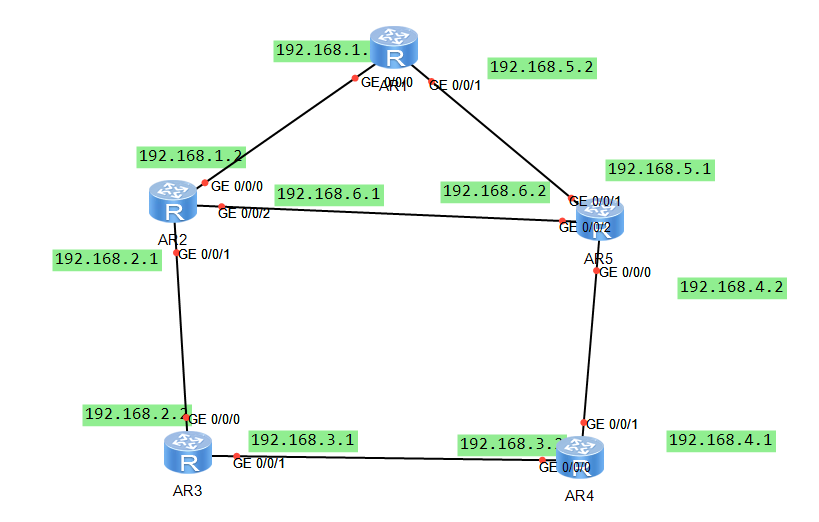
\includegraphics[width=0.6\textwidth]{topo.png}
\end{figure}

点击启动按钮,启动网络。发现各链路上的两个红点都变成绿色,证明连通。

\subsection{任务1.2}

首先,为各个路由器启用RIP协议,然后在AR1的\texttt{GE 0/0/0}端口抓包,
如图~\ref{fig:ar1rip}。

\begin{figure}[htbp]
	\centering
	\caption{RIP协议收敛过程}
	\label{fig:ar1rip}
	\begin{subfigure}{0.4\textwidth}
		\centering
		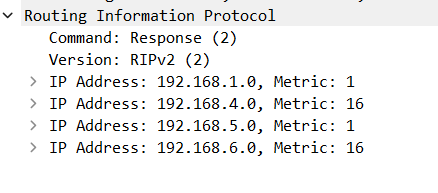
\includegraphics[width=\textwidth]{before.png}
		\caption{开始时}
		\label{fig:ar1before}
	\end{subfigure}
	\begin{subfigure}{0.4\textwidth}
		\centering
		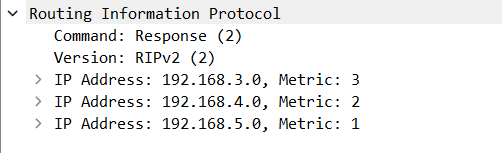
\includegraphics[width=\textwidth]{after.png}
		\caption{一段时间后}
		\label{fig:ar1after}
	\end{subfigure}
\end{figure}

一开始时,如图~\ref{fig:ar1before},有一些路由表中的距离为16,这是因为RIP协议的不可达距离为16。
经过一段时间的交换信息,可以发现交换的包中的距离已经变成拓扑图~\ref{fig:riptopo}中相应距离的
跳数。这证明算法得到了收敛。

此外,RIP协议还会定时交换路由信息。可以发现与AR1的\texttt{GE 0/0/0}
端口相连的路由器AR2的\texttt{GE 0/0/0}端口会发送Request命令UDP报文,
之后就会得到AR1的回复,如图~\ref{fig:ar2req}。
\begin{figure}[htb]
	\centering
	\caption{Request}
	\label{fig:ar2req}
	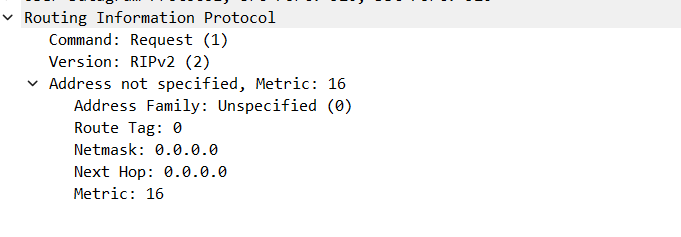
\includegraphics[width=0.5\textwidth]{request.png}
\end{figure}

在eNSP中,RIP协议的Split-horizon功能是默认启用的。因此可以观察到,AR3由于要通过AR4到达
AR5的\texttt{GE 0/0/0}端口的\texttt{192.168.4.0/32}网段。因此,AR3给AR4发送的路由信息中
不包含这一条信息,以免造成回路。如图~\ref{fig:ar3rip}。
\begin{figure}[htb]
	\centering
	\caption{Split-horizon}
	\label{fig:ar3rip}
	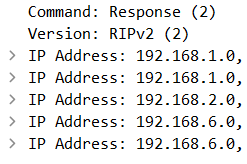
\includegraphics[width=0.3\textwidth]{sh.png} 
\end{figure}

\section{任务2}

水平分割可以防止产生回路,一定程度上缓解Count-to-infinity问题。但是,水平分割也会造成路由欺骗等问题。
在eNSP中水平分割默认开启。使用shutdown命令关闭AR2的\texttt{GE 0/0/1}端口。此时该端口的绿色点变红,
说明已经进入关闭状态。这时观察抓到的包。如图~\ref{fig:ncti}。可见,AR1和AR2仅通过两次交换就能获取不可达
的路由信息。
\begin{figure}[htbp]
	\centering
	\caption{关闭AR2后的路由信息}
	\label{fig:ncti}
	\begin{subfigure}{0.4\textwidth}
		\centering
		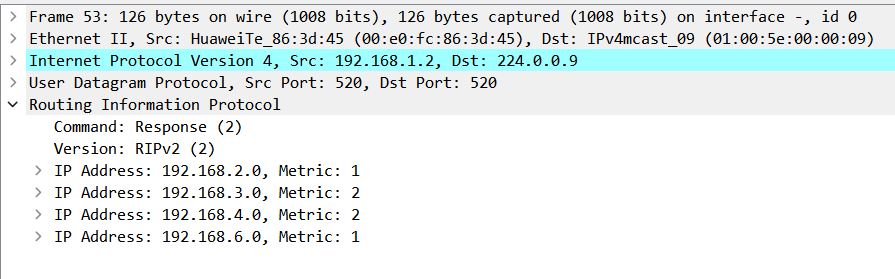
\includegraphics[width=\textwidth]{s1.png}
		\caption{第一次}
		\label{fig:ncti1}
	\end{subfigure}
	\begin{subfigure}{0.4\textwidth}
		\centering
		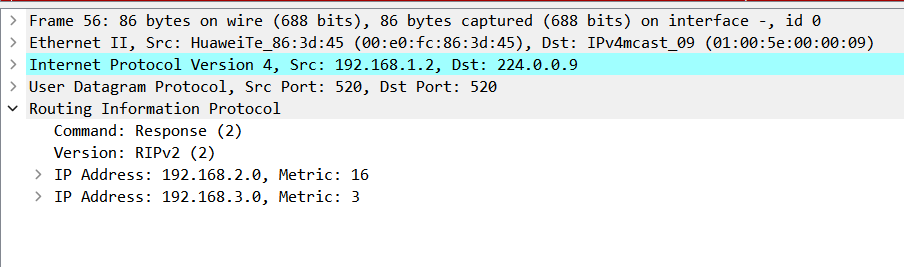
\includegraphics[width=\textwidth]{s16.png}
		\caption{第二次}
		\label{fig:ncti2}
	\end{subfigure}
\end{figure}

同样地,使用命令关闭水平逆转,再按以上操作观察结果。我们可以发现断开连接时AR1和AR2交换的包显著增加了。
这是因为水平逆转功能关闭后,AR1和AR2之间的路由信息交换不再受到Split-horizon的限制,
因此产生了Count-to-infinity问题。如图~\ref{fig:cti}。可以发现,
图~\ref{fig:cti1}到图~\ref{fig:cti13}记录到了在\texttt{192.168.1.1}和\texttt{192.168.1.2}
交换的路由信息中,Metric从1依次增大变到32的过程。
其中不仅产生了大量的路由信息交换,还造成了路由表中的路由信息不准确、收敛时间变长。

\begin{figure}[bp]
	\centering
	\caption{Count-to-infinity}
	\label{fig:cti}
	\begin{subfigure}{0.4\textwidth}
		\centering
		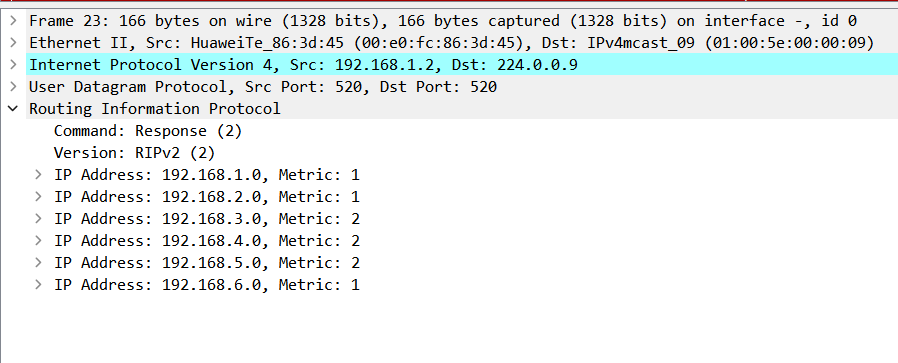
\includegraphics[width=0.9\textwidth]{1.png}
		\caption{1}
		\label{fig:cti1}
	\end{subfigure}
	\begin{subfigure}{0.4\textwidth}
		\centering
		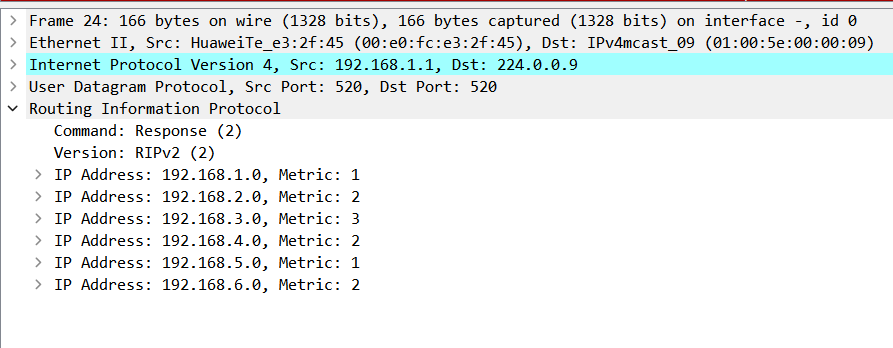
\includegraphics[width=0.9\textwidth]{2.png}
		\caption{2}
		\label{fig:cti2}
	\end{subfigure}
	\begin{subfigure}{0.4\textwidth}
		\centering
		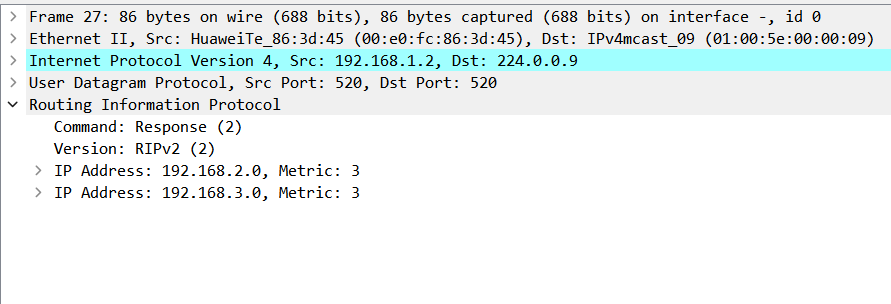
\includegraphics[width=0.9\textwidth]{3.png}
		\caption{3}
		\label{fig:cti3}
	\end{subfigure}
	\begin{subfigure}{0.4\textwidth}
		\centering
		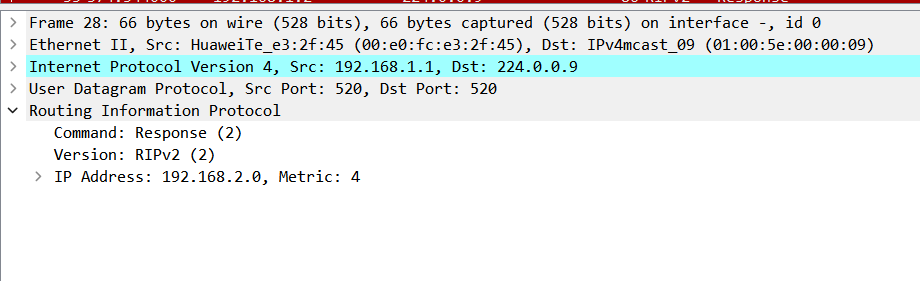
\includegraphics[width=0.9\textwidth]{4.png}
		\caption{4}
		\label{fig:cti4}
	\end{subfigure}
	\begin{subfigure}{0.4\textwidth}
		\centering
		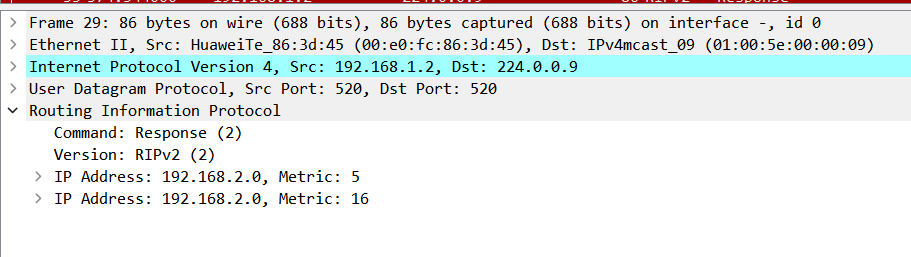
\includegraphics[width=0.9\textwidth]{5.png}
		\caption{5}
		\label{fig:cti5}
	\end{subfigure}
	\begin{subfigure}{0.4\textwidth}
		\centering
		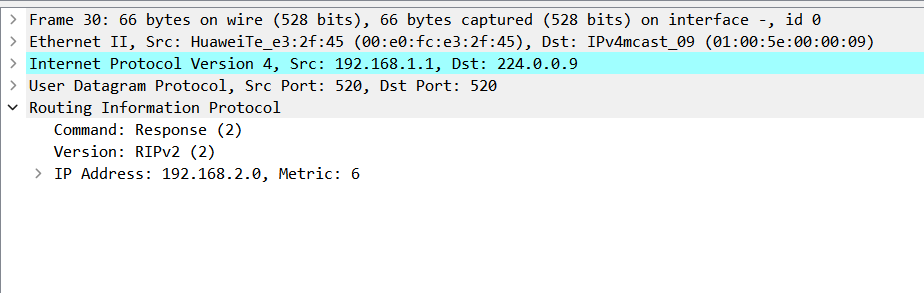
\includegraphics[width=0.9\textwidth]{6.png}
		\caption{6}
		\label{fig:cti6}
	\end{subfigure}
	\begin{subfigure}{0.4\textwidth}
		\centering
		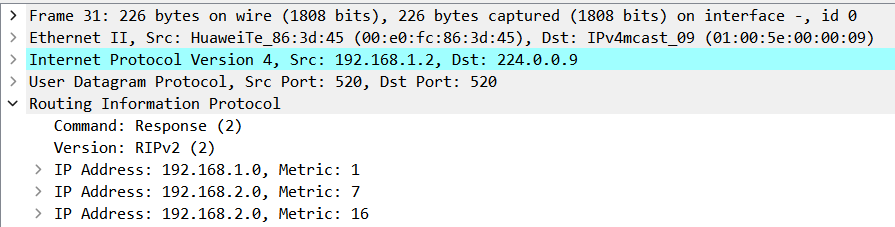
\includegraphics[width=0.9\textwidth]{7.png}
		\caption{7}
		\label{fig:cti7}
	\end{subfigure}
	\begin{subfigure}{0.4\textwidth}
		\centering
		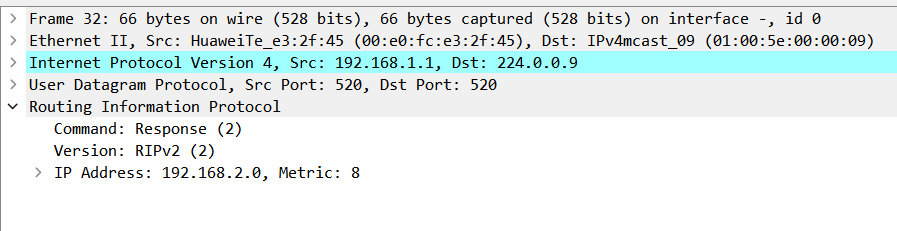
\includegraphics[width=0.9\textwidth]{8.png}
		\caption{8}
		\label{fig:cti8}
	\end{subfigure}
	\begin{subfigure}{0.4\textwidth}
		\centering
		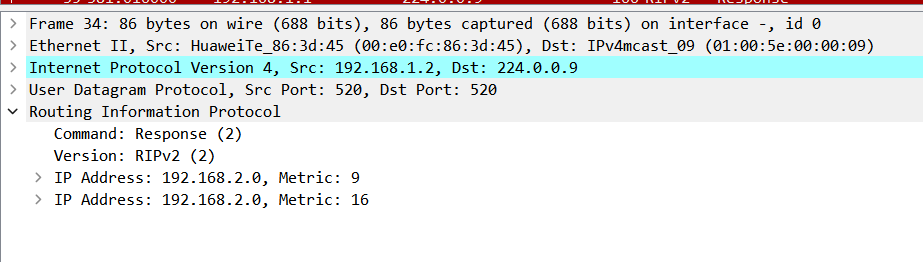
\includegraphics[width=0.9\textwidth]{9.png}
		\caption{9}
		\label{fig:cti9}
	\end{subfigure}
	\begin{subfigure}{0.4\textwidth}
		\centering
		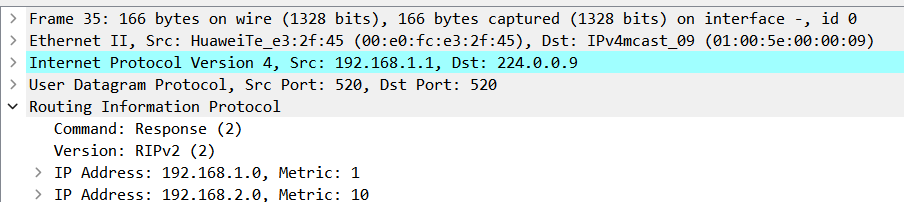
\includegraphics[width=0.9\textwidth]{10.png}
		\caption{10}
		\label{fig:cti10}
	\end{subfigure}
	\begin{subfigure}{0.4\textwidth}
		\centering
		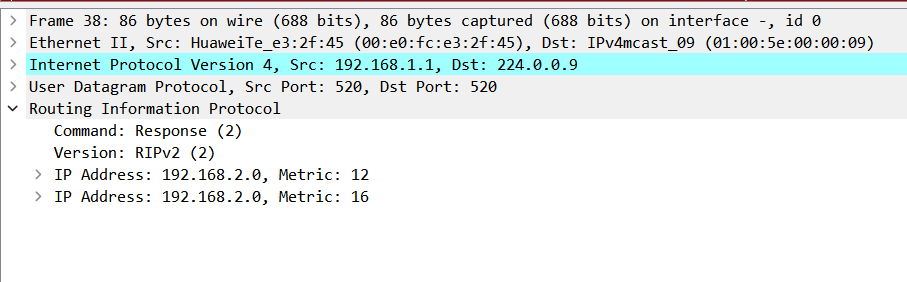
\includegraphics[width=0.9\textwidth]{11.png}
		\caption{11}
		\label{fig:cti11}
	\end{subfigure}
	\begin{subfigure}{0.4\textwidth}
		\centering
		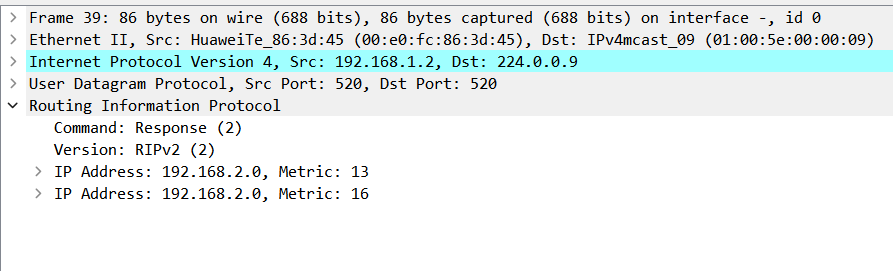
\includegraphics[width=0.9\textwidth]{12.png}
		\caption{12}
		\label{fig:cti12}
	\end{subfigure}
	\begin{subfigure}{0.4\textwidth}
		\centering
		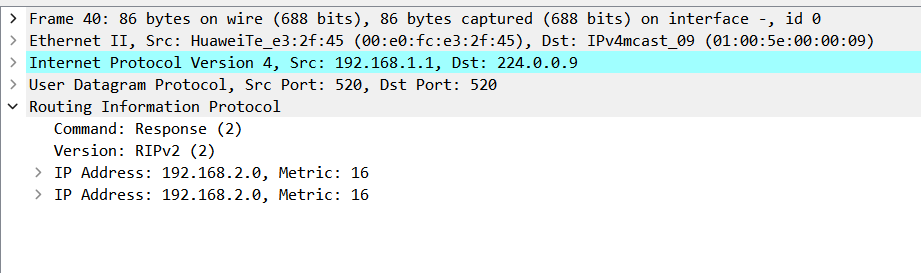
\includegraphics[width=0.9\textwidth]{13.png}
		\caption{13}
		\label{fig:cti13}
	\end{subfigure}
\end{figure}

这说明了进行Split-horizion是对RIP协议的重要优化,可以提高效率并且避免产生问题。

\section{任务3}

首先按照图~\ref{fig:riptopo}搭建网络。启动设备然后配置OSPF协议,链路上
红点变为绿色,证明连通。

在AR3的\texttt{GE 0/0/1}端口抓包,可以发现使用OSPF协议的路由器接入时会发出包表明自己已经连入网络
,并且请求链路状态。如图~\ref{fig:ospfinit}。
\begin{figure}[H]
	\centering
	\caption{OSPF启动}
	\label{fig:ospfinit}
	\begin{subfigure}{0.4\textwidth}
		\centering
		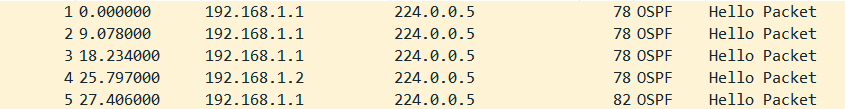
\includegraphics[width=\textwidth]{hello.png}
		\caption{Hello}
		\label{fig:hello}
	\end{subfigure}
	\begin{subfigure}{0.4\textwidth}
		\centering
		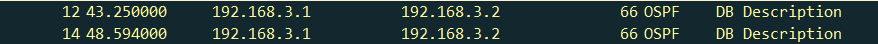
\includegraphics[width=\textwidth]{dbd.png} 
		\caption{DB Description}
		\label{fig:dbdesc}
	\end{subfigure}
\end{figure}

OSPF使用Hello分组建立和维护邻接关系。因此路由器进入网络就会不断发送Hello包。如图~\ref{fig:hello}。
DB Description分组不包含完整的“链路状态数据库”信息,只包含数据库中每个条目的概要。
当一个路由器首次连入网络,或者刚刚从故障中恢复时,它需要完整的“链路状态数据库”信息。此时,该路由器首先通过hello分组与邻居们建立双向通信关系,
然后将会收到每个邻居反馈的DB Description分组。新连入的这个路由器会检查所有概要,然后发送一个或多个链路状态请求分组,取回完整的条目信息。如图~\ref{fig:dbdesc}。

收到DB Description分组后,AR3会发送一个LS Request分组,请求AR4的LSA信息。如图~\ref{fig:lsreq}。
\begin{figure}[htb]
	\centering
	\caption{LS Request}
	\label{fig:lsreq}
	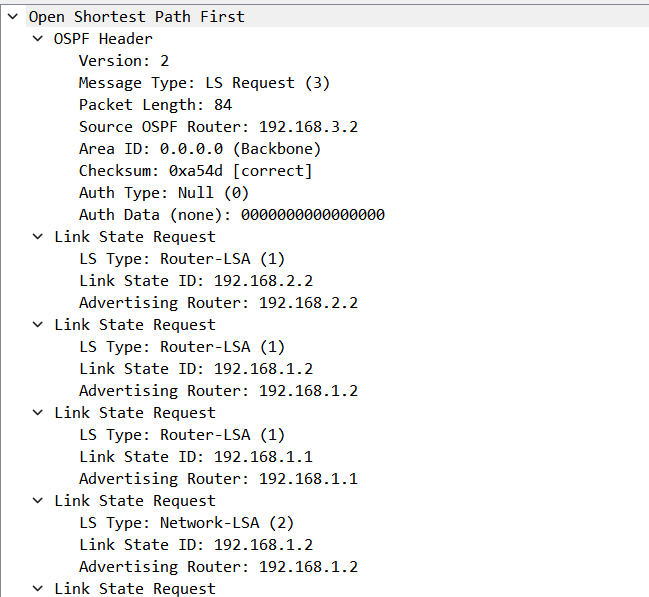
\includegraphics[width=0.4\textwidth]{lsreq.png}
\end{figure}
可见AR3向AR4请求了\texttt{192.168.1.1}、\texttt{192.168.1.2}、
\texttt{192.168.2.2}等路由器的信息。AR4收到请求后,会将这些信息发送给AR3。如图~\ref{fig:lsupdate}。
\begin{figure}[htb]
	\centering
	\caption{LS Update}
	\label{fig:lsupdate}
	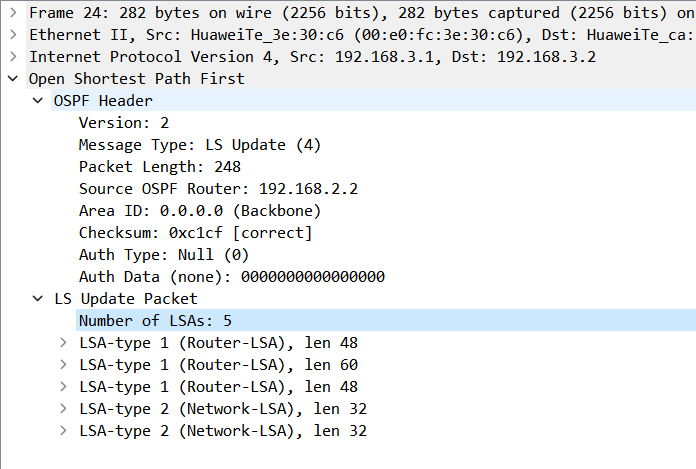
\includegraphics[width=0.4\textwidth]{lsresp.png}
\end{figure}
AR3收到LS Update分组后,会将其中的LSA信息加入到自己的数据库中。然后发出确认分组
LS Acknowledgement。如图~\ref{fig:lsack}。
\begin{figure}[htb]
	\centering
	\caption{LS Acknowledgement}
	\label{fig:lsack}
	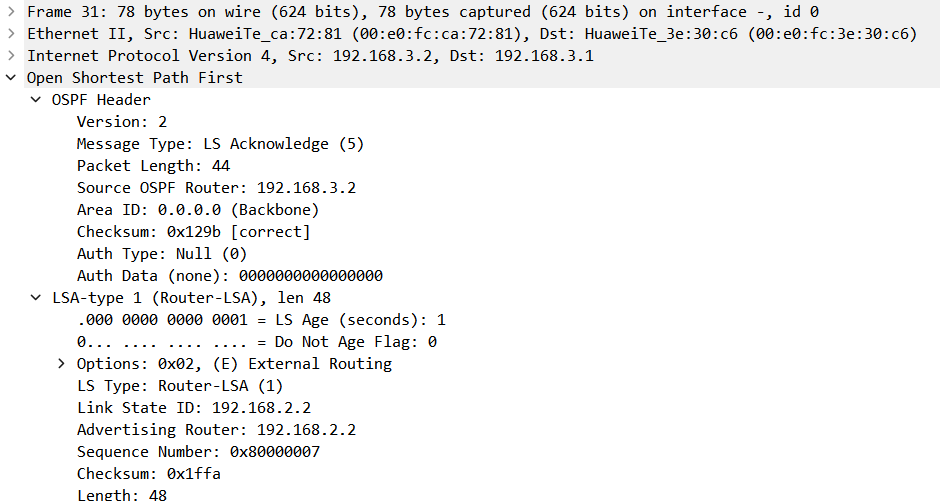
\includegraphics[width=0.4\textwidth]{lsack.png}
\end{figure}
OSPF就像这样在相邻的路由器间交换信息。

进入接口模式,将\texttt{192.168.1.1}-\texttt{192.168.1.2}的Cost改为6。
可见,AR1将会发出LS Update分组,将新的Cost信息发送给AR2。如图~\ref{fig:costchange}。
\begin{figure}[htb]
	\centering
	\caption{Cost改变}
	\label{fig:costchange}
	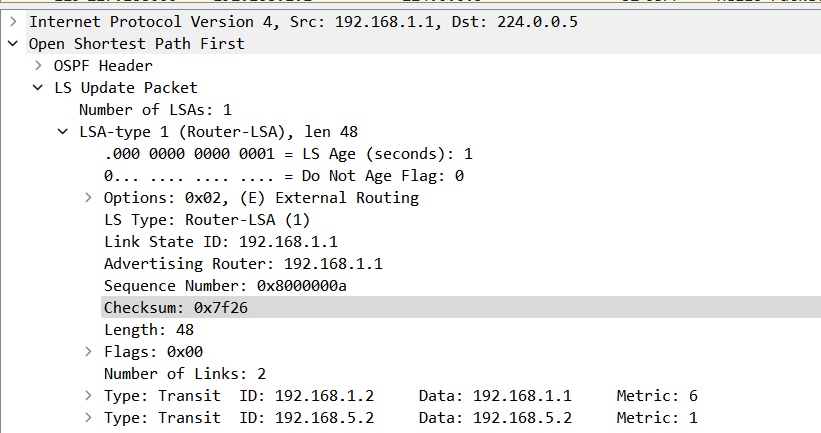
\includegraphics[width=0.4\textwidth]{inccost.png}
\end{figure}
可以发现,链路状态的Metric变为6。AR2收到后,会将新的链路状态信息发送给其相邻路由。
如图~\ref{fig:costchange2}。
\begin{figure}[htb]
	\centering
	\caption{Cost改变}
	\label{fig:costchange2}
	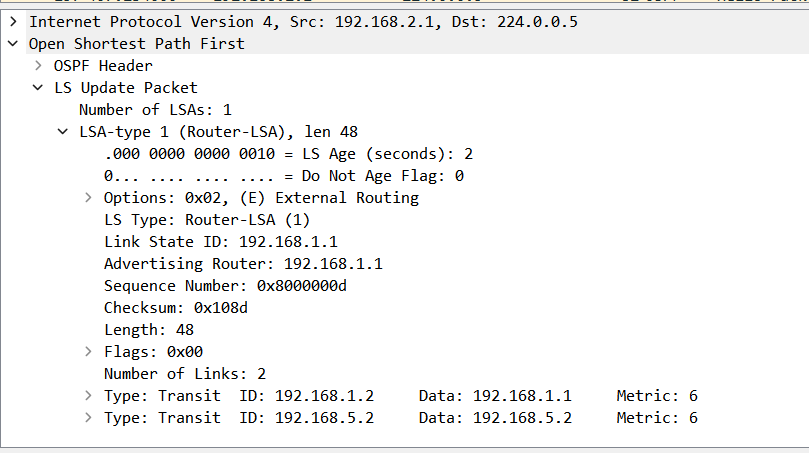
\includegraphics[width=0.4\textwidth]{22lup.png}
\end{figure}
这个数据包由AR2发给AR3,可见其中说明了AR1与AR2之间链路的Cost变为6。AR3收到后,也会将新的链路状态信息发送给其相邻路由。
这样通过可靠洪泛机制,链路状态的改变就得以在不同的路由器间传播。可以发现,整个拓扑中各路由器的链路状态
会很快收敛。最后各路由器的路由表如图~\ref{fig:rt}。
\begin{figure}[bp]
	\centering
	\caption{各路由器的路由表}
	\label{fig:rt}
	\begin{subfigure}{0.4\textwidth}
		\centering
		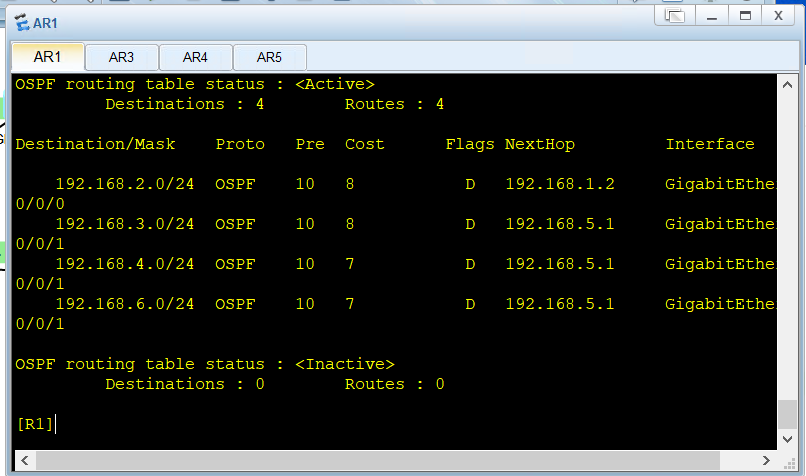
\includegraphics[width=\textwidth]{ar1.png}
		\caption{AR1}
		\label{fig:ospfar1}
	\end{subfigure}
	\begin{subfigure}{0.4\textwidth}
		\centering
		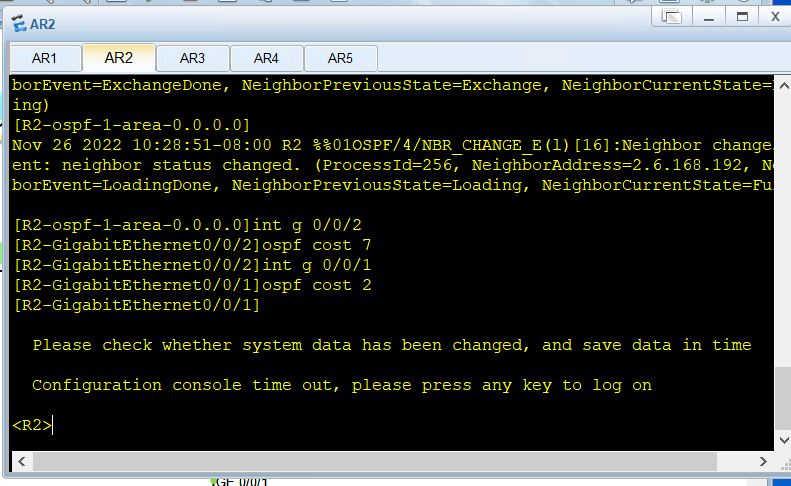
\includegraphics[width=\textwidth]{ar2.png}
		\caption{AR2}
		\label{fig:ospfar2}
	\end{subfigure}
	\begin{subfigure}{0.4\textwidth}
		\centering
		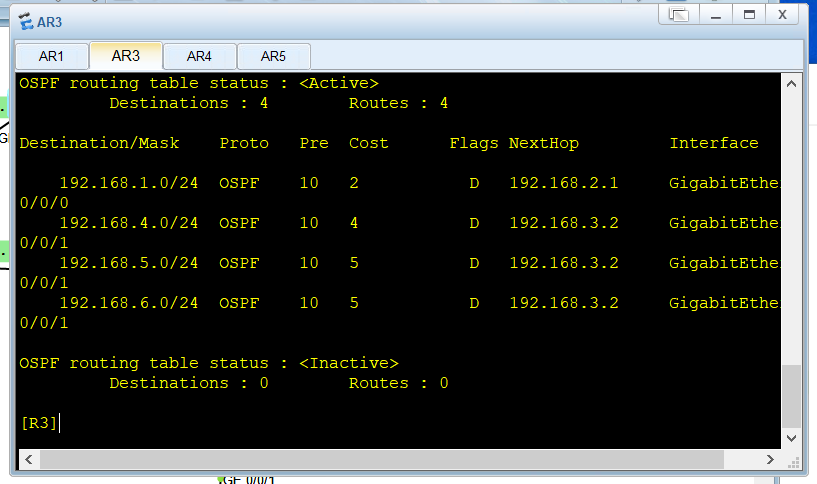
\includegraphics[width=\textwidth]{ar3.png}
		\caption{AR3}
		\label{fig:ospfar3}
	\end{subfigure}
	\begin{subfigure}{0.4\textwidth}
		\centering
		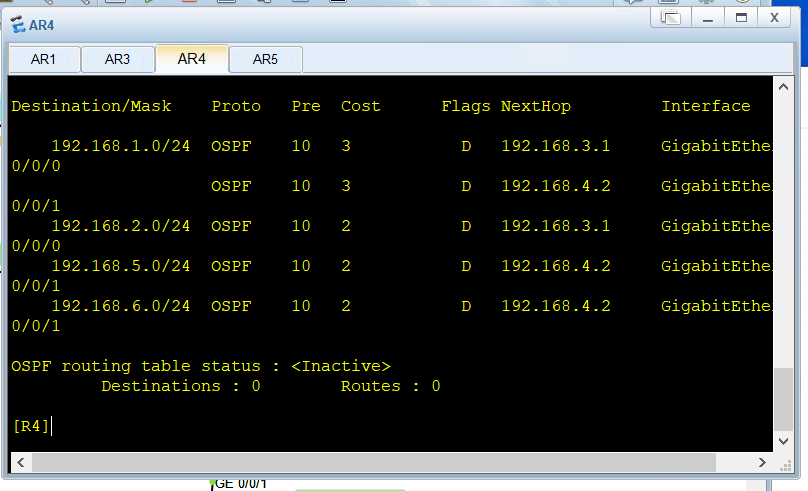
\includegraphics[width=\textwidth]{ar4.png}
		\caption{AR4}
		\label{fig:ospfar4}
	\end{subfigure}
	\begin{subfigure}{0.4\textwidth}
		\centering
		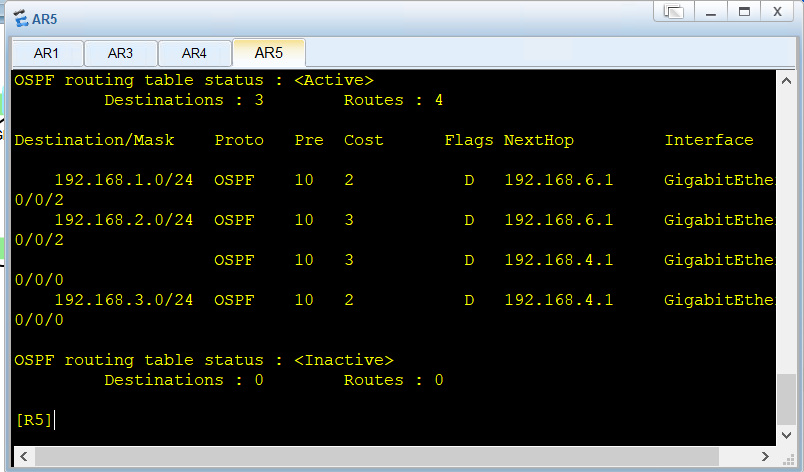
\includegraphics[width=\textwidth]{ar5.png}
		\caption{AR5}
		\label{fig:ospfar5}
	\end{subfigure}
\end{figure}

\clearpage
\section{实验总结}

在本次实验中,我观察了RIP协议和OSPF协议传递路由信息的过程。体会了RIP协议中Split-horizon策略
具有的重大意义。观察了链路状态改变时OSPF如何通过可靠洪泛机制将新的链路状态信息传播到整个拓扑中。
通过本次实验,我对RIP和OSPF协议有了更深的了解。

\end{spacing}

\end{document}